% !TEX program = xelatex
\documentclass[aspectratio=1610,multi,rgb]{beamer}

%\documentclass[12pt]{article}
%\usepackage[noxcolor]{beamerarticle}

\usepackage[edges]{forest}
\usepackage{chronology}
\usepackage{ragged2e}
\usepackage[spanish]{babel}
\usepackage{nameref}
\usepackage{multimedia}
\usepackage{pgfplots}
\usepackage{scrextend}
\usepackage{multicol}
\usepackage{geometry}
\usepackage{fontspec}
\usepackage{tabularx}
\usepackage{graphicx}
\usepackage{booktabs}
\usepackage{listings}
\usepackage{fancybox}
\usepackage{textpos}
\usepackage{xcolor}
\usepackage{subfig}
\usepackage{color}
\usepackage{calc}
\usepackage{tikz}
\usetikzlibrary{arrows.meta,shadows.blur}
\usepackage{empheq}
\usepackage[T1]{fontenc}
\usepackage{lmodern}
\usepackage[backend=biber, style=authoryear-icomp]{biblatex}


\setbeameroption{show notes}
\setbeameroption{show notes on second screen=right}

%\usetheme{Luebeck}
%\usetheme{Marburg}
%\usetheme{Goettingen}
%\usetheme{Hannover}
\usetheme{Antibes}
%\usecolortheme{whale}

\let\raggedright=\RaggedRight

%-------------------------------------------------------------------------------
\definecolor{lightgreen}{HTML}{90EE90}
\colorlet{myyellow}{yellow!50}
\usefonttheme{professionalfonts} % using non standard fonts for beamer
%\setmainfont{IBM Plex Sans}
%\setbeamertemplate{navigation symbols}{\insertlogo}
\setbeamertemplate{navigation symbols}{}
%-------------------------------------------------------------------------------

%_______Configuro el paquete de listing____
\lstset{
    inputencoding=utf8,
    extendedchars=true,
    frame=lines,
}

\definecolor{black}{rgb}{0, 0, 0}
\definecolor{codeblue}{rgb}{0,0.05,0.9}
\definecolor{codegreen}{rgb}{0,0.6,0}
\definecolor{codegray}{rgb}{0.5,0.5,0.5}
\definecolor{codepurple}{rgb}{0.58,0,0.82}
\definecolor{codeorange}{rgb}{0.7,0.2,0.1}
\definecolor{backcolour}{rgb}{0.90,0.90,0.90}


\lstdefinestyle{mystyle}{
    backgroundcolor=\color{backcolour},   
    commentstyle=\color{codepurple},
    keywordstyle=\color{codeblue},
    numberstyle=\tiny\color{codegray},
    stringstyle=\color{codeorange},
    basicstyle=\ttfamily\footnotesize\color{black},
    breakatwhitespace=false,         
    breaklines=true,                 
    captionpos=b,                    
    keepspaces=true,                 
    numbers=left,                    
    numbersep=5pt,                  
    showspaces=false,                
    showstringspaces=false,
    showtabs=false,                  
    tabsize=4
}

\lstset{style=mystyle}

\newcommand{\titleframe}[1]{
	\begin{frame} \null\hfill\huge{\shadowbox{#1}}\hspace{1cm} \end{frame}
}

\newcommand{\boxedeq}[2]{
	\begin{empheq}[box={\fboxsep=6pt\fbox}]{align}\label{#1}#2\end{empheq}
}

\newcommand{\coloredeq}[2]{
	\begin{empheq}[box=\colorbox{lightgreen}]{align}\label{#1}#2\end{empheq}
}

\newcommand{\fig}[3]{
	\begin{columns}
	\column{0.4\textwidth}
	\begin{figure}[htp] 
		\includegraphics[height=0.5\textheight,width=0.9\textwidth,
	keepaspectratio]{#1}\caption{#2}\end{figure}
	\column{0.6\textwidth}#3
	\end{columns}
}
\newcommand{\tabitem}{~~\llap{\textbullet}~~}

\newcommand{\htree}[1]{
	\begin{forest}
	for tree={
	fit=band,
	grow'=0,
	parent anchor=children,
	child anchor=parent,
	anchor=parent,
	if n children=0{folder}{},
	edge path'={(!u.parent anchor) -- ++(5pt,0) |- (.child anchor)},
	},
	where n=1{
	calign with current edge
	}{},
	#1
	\end{forest}
}

\include{beamer.tex}
\addbibresource{bibliography.bib}

\usepackage{pdfpages}

%-------------------------------------------------------------------------------
\title{Python como herramienta de automatización de cálculo}
\subtitle{Caso aplicado en envolventes trifásicas}
\author{Federico Benelli}
\institute{IPQA}
\date{\today}

\logo{
\begin{tabular}{cc}
    
\includegraphics[height=0.5cm]{figs/fcefyn-logo.png} &
    
\includegraphics[height=0.5cm]{figs/ipqa-logo.png}
\end{tabular}

% Method to add an item that will appear in every slide
\addtobeamertemplate{footline}{%
  \setlength\unitlength{1ex}%
  \begin{picture}(0,0) 
    % \put{} defines the position of the frame
    \put(140,6){\makebox(0,0)[bl]{
        
\includegraphics{figs/fcefyn-logo.png}
        
\includegraphics{figs/ipqa-logo.png}
    }}%
  \end{picture}%
}{}
}
%-------------------------------------------------------------------------------

\begin{document}
\nocite{*} % Show everything in bibliography file, even not cited

\begin{frame}\maketitle\end{frame}
\begin{frame}\tableofcontents\end{frame}

\section{Introducción}\label{intro}
\subsection{Descripción del problema}\label{prob}

\begin{frame}[c]
    \frametitle{Introducción}
    \framesubtitle{Descripción del problema}

    \begin{columns}
        \column{0.5\textwidth}
        \begin{figure}[htpb]
            \centering
            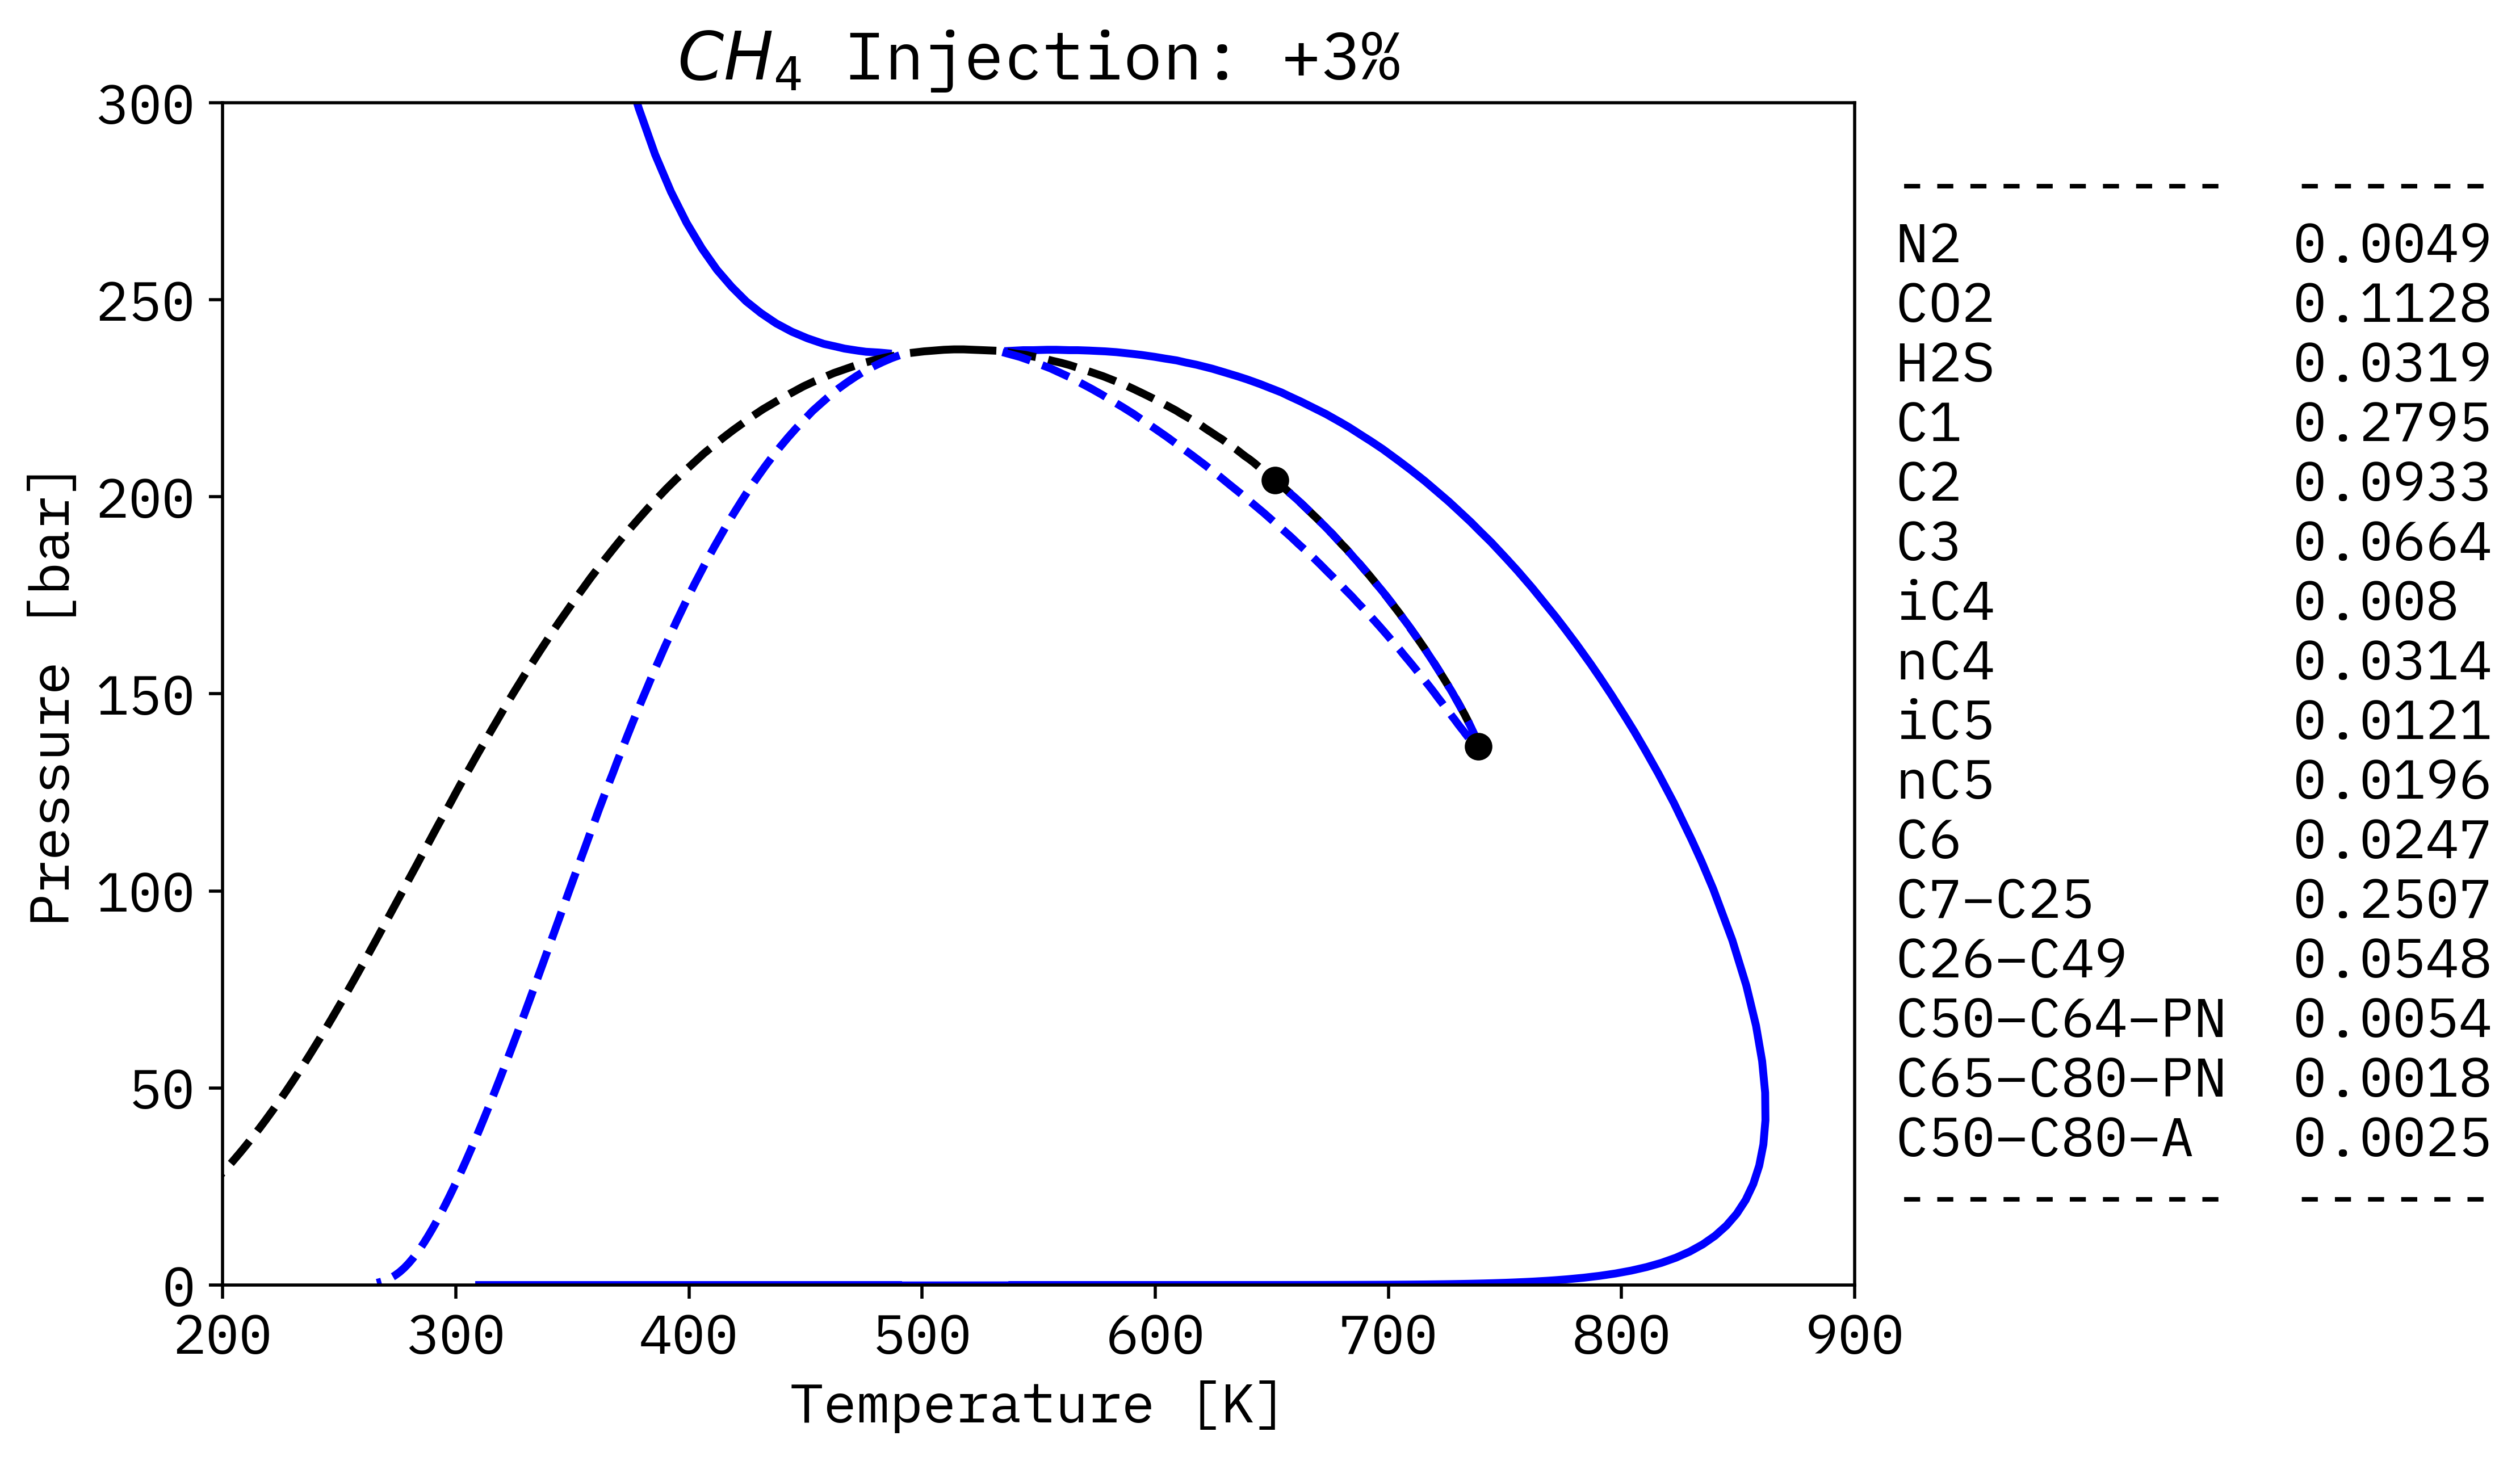
\includegraphics[width=0.9\textwidth]{figs/envelope1.png}
            \caption{}
            \label{fig:figs-envelope1-png}
        \end{figure}

        \column{0.5\textwidth}
        \begin{figure}[htpb]
            \centering
            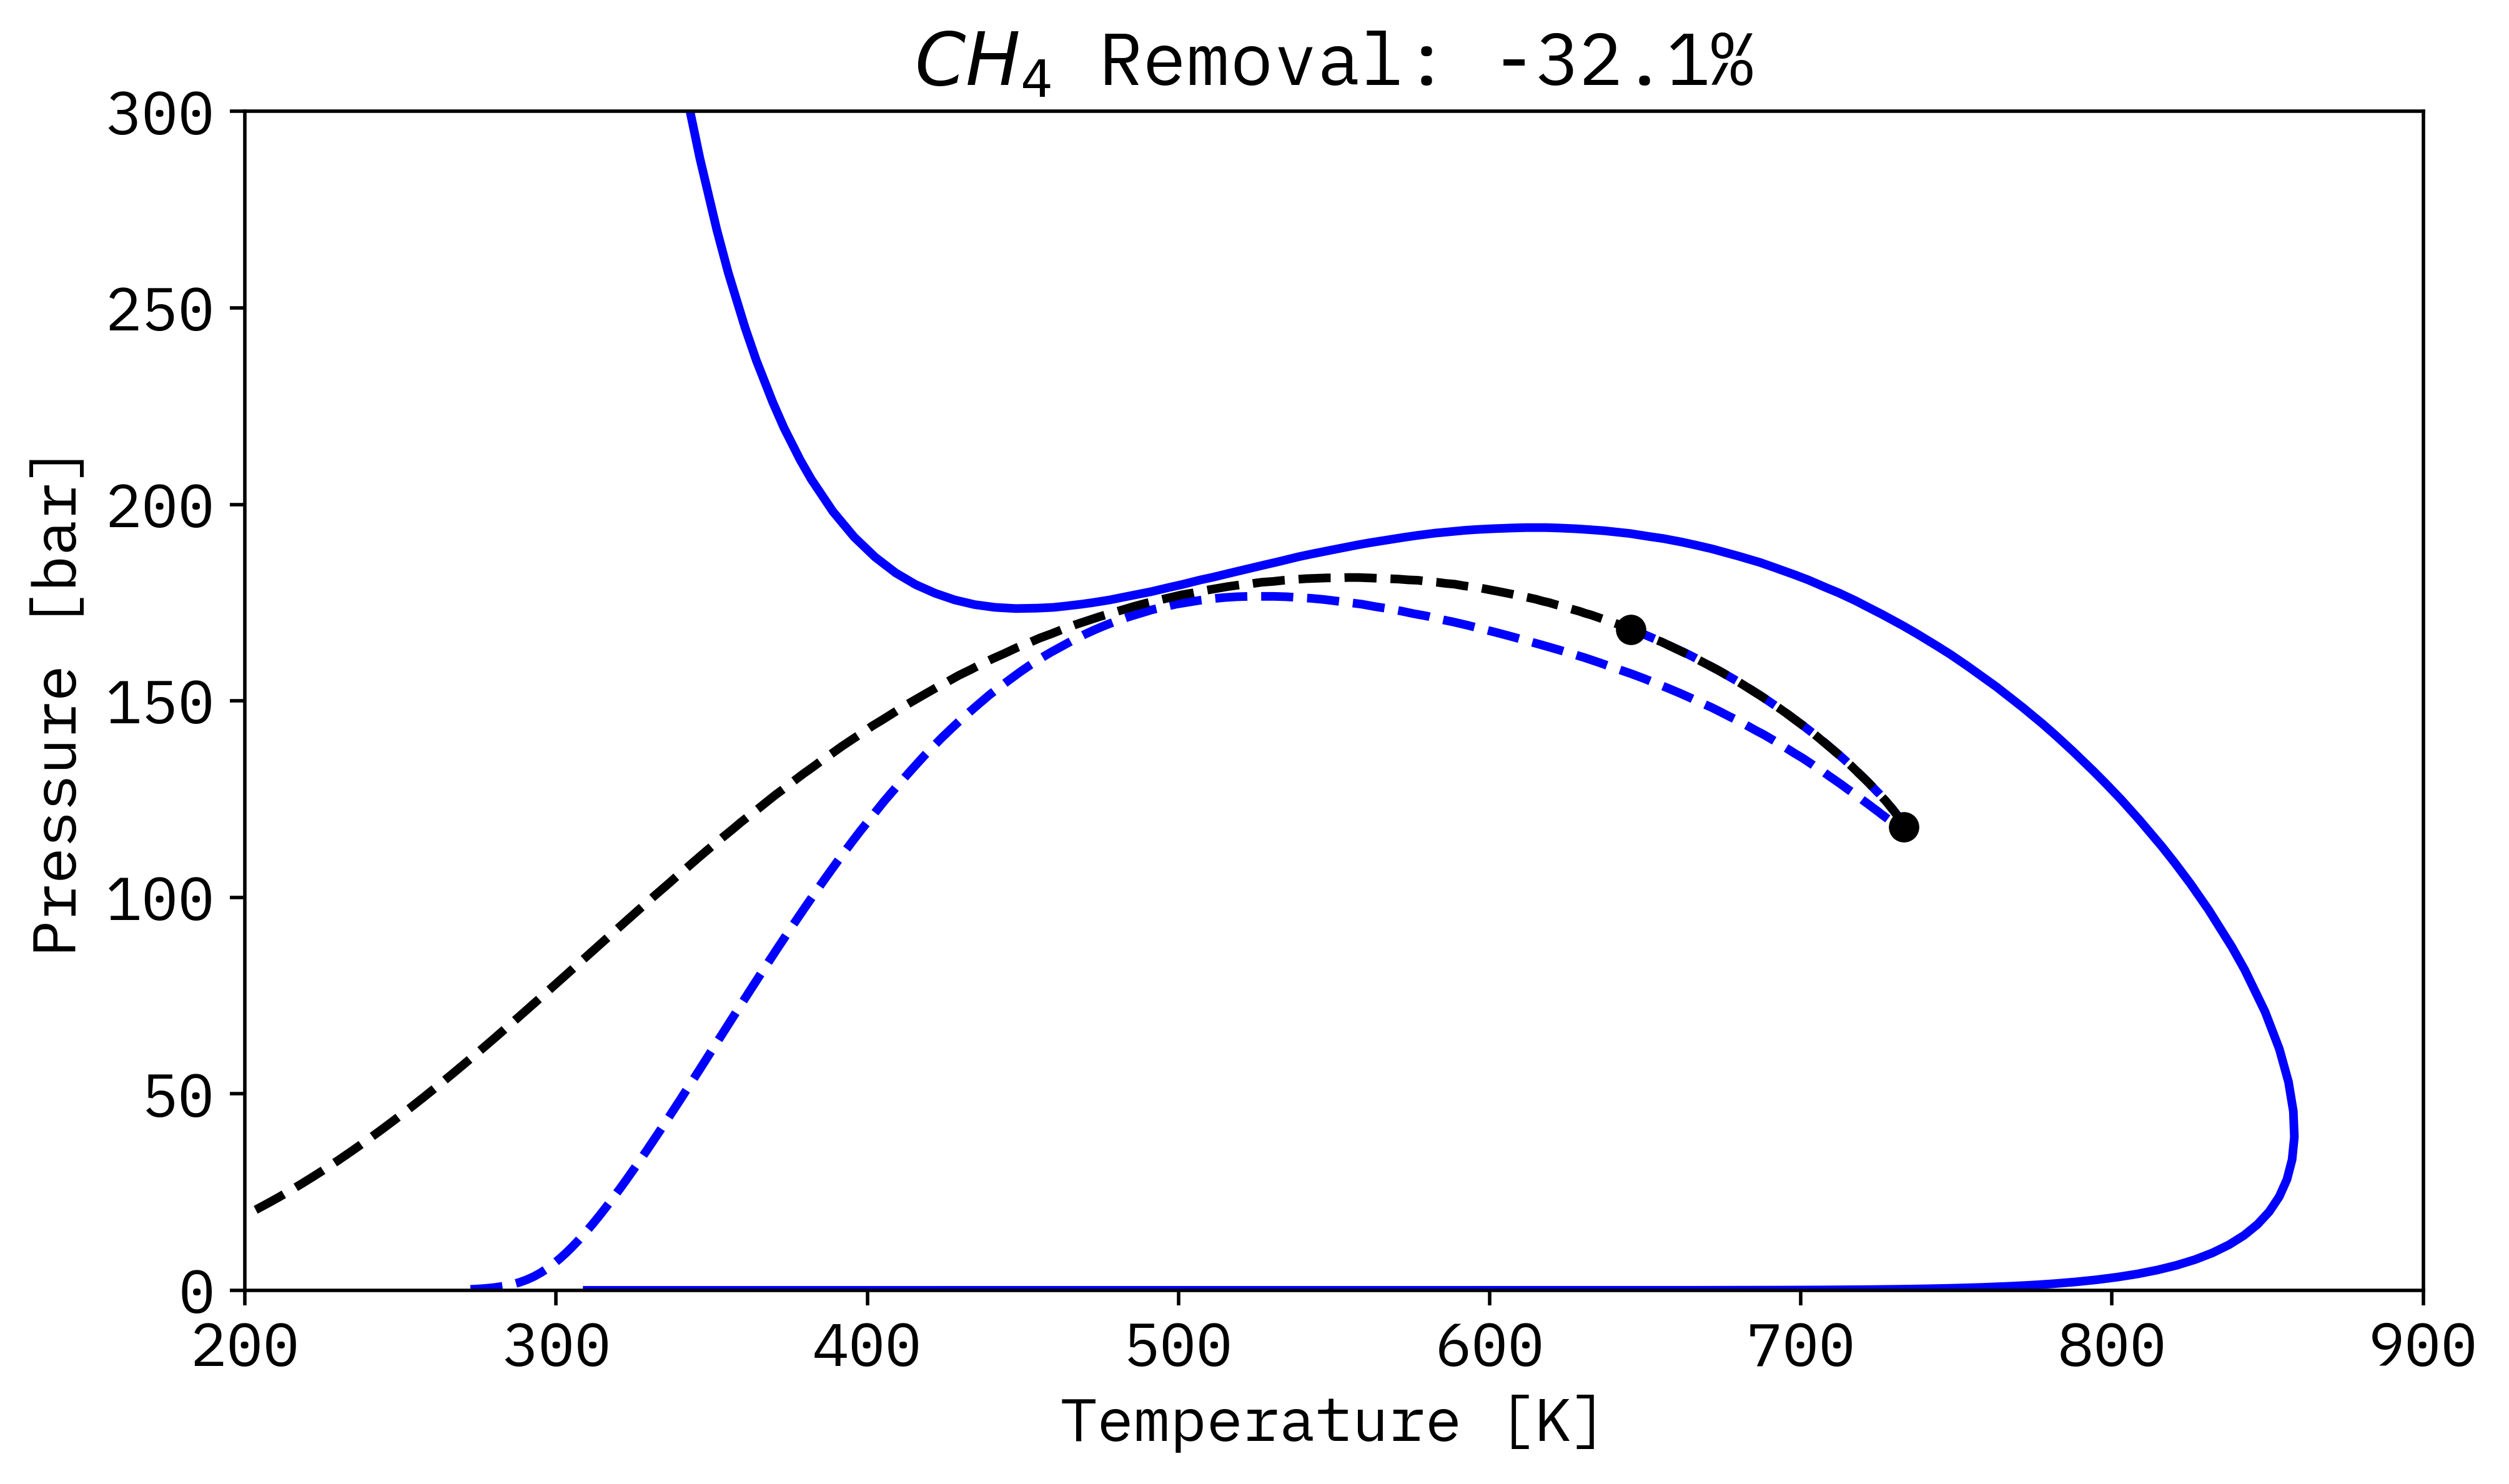
\includegraphics[width=0.9\textwidth]{figs/envelope2.png}
            \caption{}
            \label{fig:figs-envelope1-png}
        \end{figure}
    \end{columns}

    \note{En un congreso reciente se presentó un trabajo consistente en la
    categorización de casos particulares de sistemas multicomponentes con prenencia
    de equilibrios trifásicos.

    Para poder realizar esta categorización fue necesario realizar múltiples
    ejecuciones de un programa que calcula las envolventes correspondientes.
    }

    Problema: Necesidad de generar y correr múltiples casos en un tiempo
    relativamente acotado.
    
\end{frame}

\subsection{Programa original}\label{forprog}
\begin{frame}[c]
    \frametitle{Programa original}
    \framesubtitle{Descripción}
    \note{
    Para el cálculo de estas envolventes se utilizó un programa previamente
    desarrollado, con unas modificaciones básicas para facilitar la
    automatización del proceso de generación de gráficos.
    }
    \begin{figure}[htpb]
        \centering
        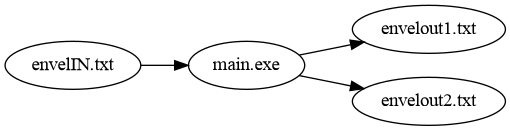
\includegraphics[width=0.7\textwidth]{figs/orig.png}
        \caption{Funcionamiento básico programa}
    \end{figure}
\end{frame}

\subsubsection{Archivo de entrada}
\begin{frame}[c, fragile]
    \frametitle{Introducción}
    \framesubtitle{Archivos de entrada}
    \note{
     El programa que realiza los cálculos utiliza como input archivos de texto
    simple con una estructura predefinida. El archivo debe llamarse
    envelin y encontrarse en la misma carpeta que el ejecutable.
    }

    \texttt{envelIN.txt}

\begin{lstlisting}
 15     NC Fluid A Jamaluddin 2000 (Table 12.8 Pedersen)
 0.0048 0.00919 0.43391 0.1101 0.06544 0.00789 0.03787 0.01279 ...
 2      NMODEL (1:SRK / 2:PR / 3:RKPR)
 0  0   ncomb, nTdep
 N2  
  126.2000   33.9400  0.040000  0.09504
    1.4833  0.024051  0.435899
 CO2 
  304.2000   73.7600  0.225000  0.10541
    3.9656  0.026677  0.707984
 -0.032  kij
  0.0    lij
  ...
\end{lstlisting}
    
\end{frame}


\subsubsection{Archivo de salida}

\begin{frame}[c, fragile]
    \frametitle{Introducción}
    \framesubtitle{Archivos de salida}
\note{
    Tras la ejecución, el programa genera un archivo de salida por cada envolvente
    calculada. Llamados \texttt{envelout<N>.txt}
}
\texttt{envelout3.txt}
\begin{lstlisting}
    T(K)        P(bar)        D(mol/L)
    310.0000    0.1529E-23    0.5930E-25
    311.5589    0.2517E-23    0.9715E-25
    313.7960    0.5098E-23    0.1954E-24
    316.0554    0.1028E-22    0.3912E-24
    318.3371    0.2065E-22    0.7801E-24
    ...

  Number of critical points found:            1
    T(K)        P(bar)        D(mol/L)
    639.1631    0.2328E+03    0.4516E+01  225
\end{lstlisting}
    
\end{frame}

\section{Definición de casos de estudio}\label{casosestudios}
\begin{frame}[c]
    \frametitle{Definición de casos de estudio}

    Se partió de los tres casos de estudio originales, a partir de los cuales se
    generaron variantes.

    \begin{columns}
        \column{0.3\textwidth}
        \begin{figure}[htpb]
            \centering
            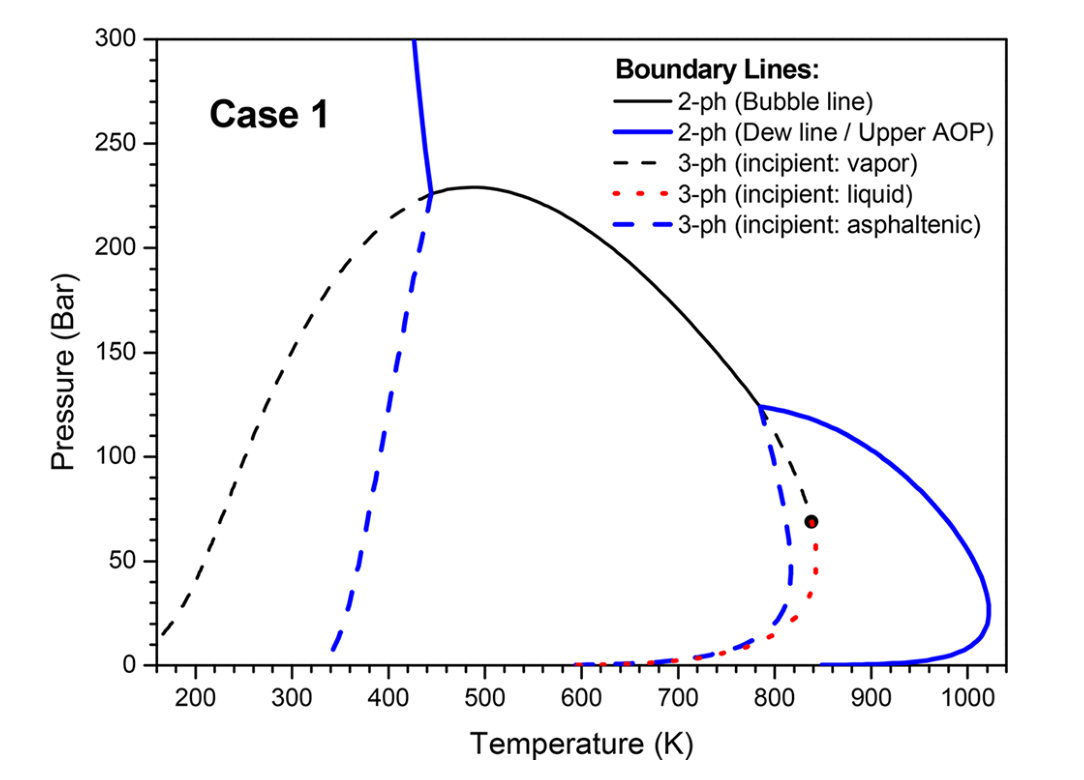
\includegraphics[width=0.9\textwidth]{figs/case1.png}
            \caption{Caso 1}
            \label{fig:case2}
        \end{figure}
        \column{0.3\textwidth}
        \begin{figure}[htpb]
            \centering
            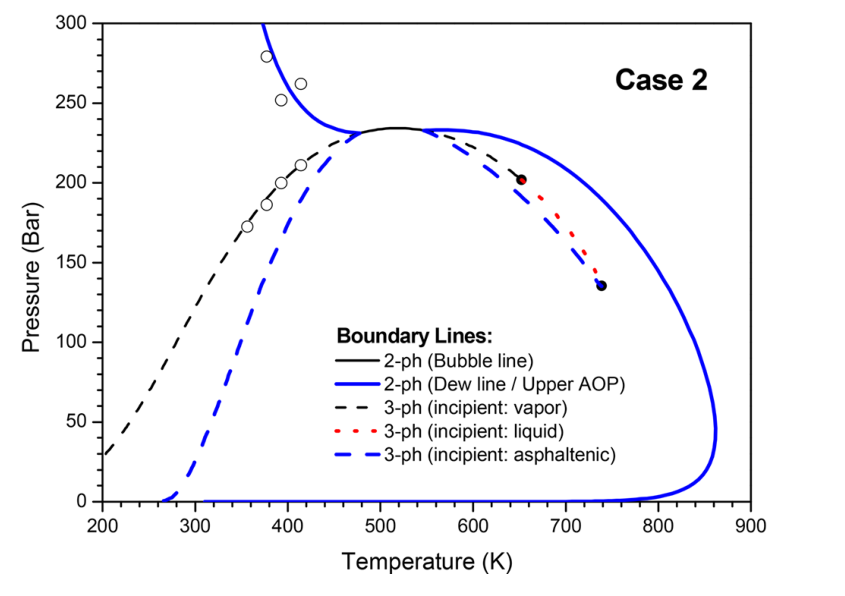
\includegraphics[width=0.9\textwidth]{figs/case2.png}
            \caption{Caso 2}
            \label{fig:case2}
        \end{figure}
        \column{0.3\textwidth}
        \begin{figure}[htpb]
            \centering
            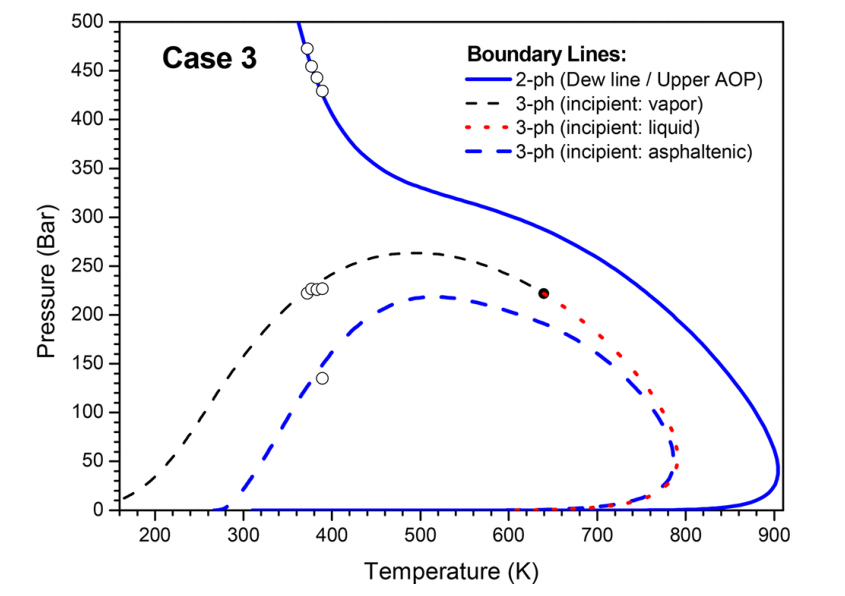
\includegraphics[width=0.9\textwidth]{figs/case3.png}
            \caption{Caso 3}
            \label{fig:case3}
        \end{figure}
    \end{columns}
\end{frame}

\subsection{Metodología}\label{met}
\begin{frame}[c]
    \frametitle{Metodología}

    Definir rangos!

    \note{
    Fue necesario definir un gran número de casos de estudio, con el fin de barrer
    la mayor cantidad posibles combinaciones (lógicas).

    Para esto se generaron archivos Excel con los rangos de concentraciones a
    estudiar. (Captura Excel)}

    \begin{figure}[htpb]
        \centering
        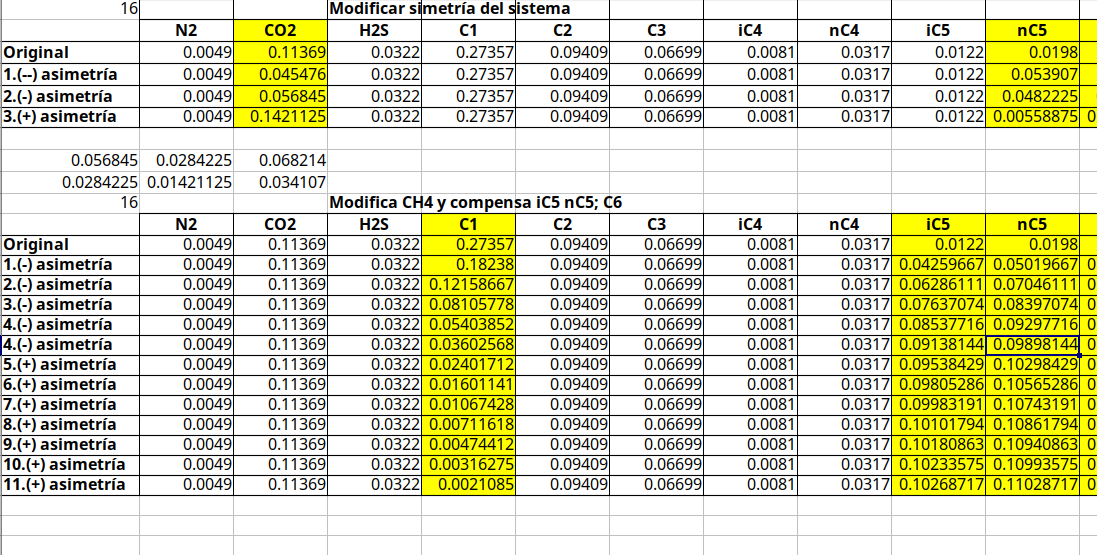
\includegraphics[width=0.8\textwidth]{figs/excel.png}
        \caption{Archivo Excel}
        \label{fig:figs-excel-png}
    \end{figure}
\end{frame}

\section{Resolución en Python}
\begin{frame}[c]
    \frametitle{Resolución en Python}
    \framesubtitle{Introducción}
    \note{
        Se desarrolló un pequeño script en Python para automatizar todo el proceso de
        generación de gráficos para su posterior análisis.
    }
    \begin{figure}[htpb]
        \centering
        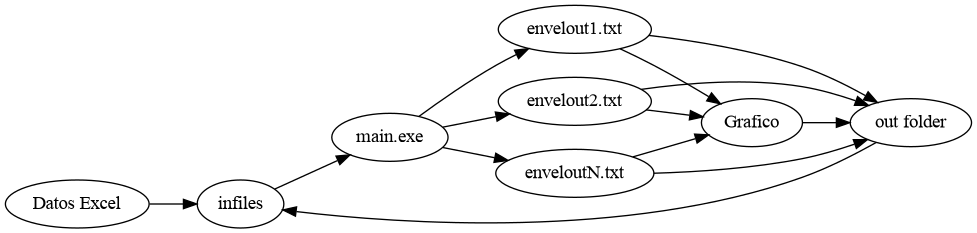
\includegraphics[width=0.8\textwidth]{figs/script.png}
        \caption{Esquema general}
        \label{fig:}
    \end{figure}
\end{frame}


\subsection{Lectura de archivos Excel}

\begin{frame}[c]
    \frametitle{Resolución en Python}
    \framesubtitle{Lectura de datos en Excel}
    \note{
    Para la lectura de archivos Excel, se utilizó la librería \texttt{openpyxl},
    la cual permite la rápida lectura.
    En cada archivo Excel se iteró por filas, identificando el comienzo de cada
    tabla, leyendo su título correspondiente.
    }
    \textit{Estructura de tabla}:
    \begin{itemize}
        \item Número de compuestos.
        \item Título.
        \item Etiqueta de fila.
        \item Concentraciones.
    \end{itemize}

    \begin{figure}[htpb]
        \centering
        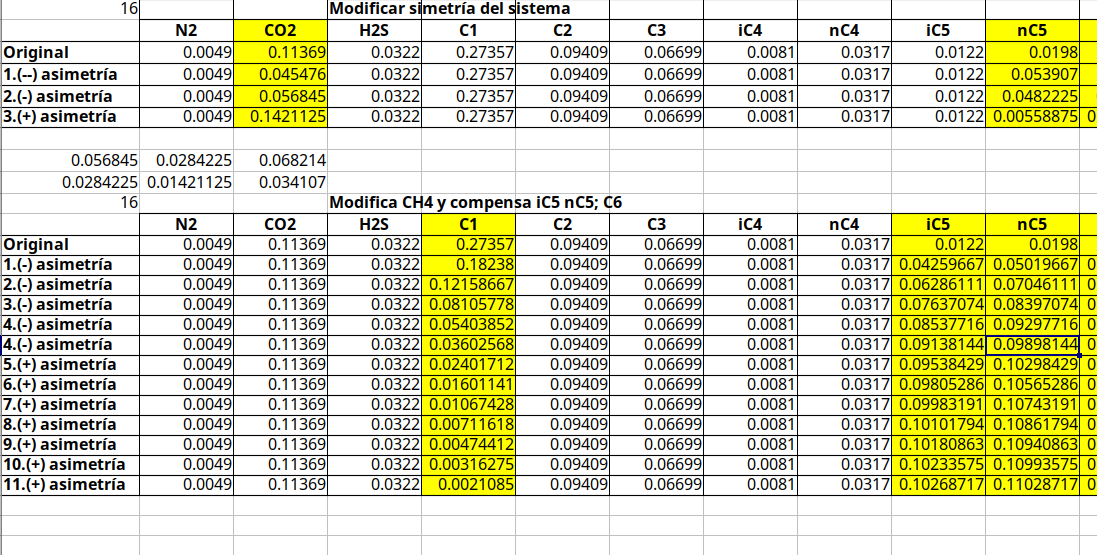
\includegraphics[width=0.5\textwidth]{figs/excel.png}
        \caption{}
        \label{fig:figs-excel-png}
    \end{figure}
\end{frame}

\subsection{Generación de archivos}

\begin{frame}[c]
    \frametitle{Resolución con Python}
    \framesubtitle{Generación archivos}

    Durante la lectura del archivo Excel se realizaron los chequeos y acciones.
    
    \begin{itemize}
        \item En tabla? -> Crear carpeta \texttt{outfiles/nombretabla}
        \item Fila con contenido? ->
            \begin{itemize}
                \item Leer concentraciones
                \item Modificar archivo input con las nuevas concentraciones
                \item Copiar nuevo archivo input a \texttt{outfiles/nombretabla/caso.archivonuevo}
            \end{itemize}
    \end{itemize}

\end{frame}

\begin{frame}[c]
    \frametitle{Resolución con Python}
    \framesubtitle{Generación de archivos de entrada}
    
    Finalizada la lectura de el archivo se obtiene una estructura de archivos de entrada como:
    \htree{
        [inputs,
        [Modifica CH4 y compensa iC5 nC5; C6,
            [(+) asimetría]
            [(- -) asimetría]
            [(-) asimetría]
        ]
        [Modifica CO2 y compensa iC5 nC5 C6,
            [(+) asimetría]
            [(- -) asimetría]
            [(-) asimetría]
        ]
        ]
    }
\end{frame}

\subsection{Ejecución de programa Fortran}
\begin{frame}[c, fragile]
    \frametitle{Resolución con Python}
    \framesubtitle{Ejecución de compilado Fortran}

\note{Una vez con todos los archivos de salida generados, es necesario ejecutar
el programa Fortran. Al ser una aplicación de consola, es un paso sencillo
donde se puede ejecutar como un comando de sistema}

\begin{lstlisting}[language=Python]
 def run_fortran(i, out_dir):
     """Función run_fortran, recibe un número de iteración y 
     un directorio de salida"""

     os.system("./main.exe")

     # Juntar todos los archivos de salida en una lista
     envelopes = sorted(glob("envelout*"))

     # envelopes = ["envelout1.txt", "envelout2.txt", ...]
     ...
\end{lstlisting}
\end{frame}

\subsection{Generación de gráfico}
\begin{frame}[c, fragile]
    \frametitle{Resolución con Python}
    \framesubtitle{Generación de gráfico}
    \note{Una vez con los archivos de salida, se llama a una función que recibe estos
    nombres y un nombre de gráfico.}
\begin{lstlisting}[language=python]
 ...
 # Funcion make_figure -> Recibe la lista de envolventes y 
 #  el titulo a darle al grafico
 make_figure(envelopes, title='\n'.join(out_dir.split("/")[-2:]))
\end{lstlisting}
\end{frame}

\begin{frame}[fragile]
    \frametitle{Generación de gráficos}
    \framesubtitle{Función make figure}
    
    \note{
    Dentro de la función make figure se itera por cada archivo, para el cual
    se llama a la función plot envelope, la cual realiza la lectura de los
    datos en el archivo y traza la línea correspondiente.
    }


\begin{lstlisting}[language=python]
def make_figure(envelopes, title):
    """From a set of envelopes, plot them."""
    plt.clf()

    for i, file in enumerate(envelopes):
        ax = plt.subplot()
        show_crit(file, '', ax)
        if i == 0:
            plot_envelope(file, 'dew', ax)
        elif i == 1:
            plot_envelope(file, 'bub', ax)
        elif i > 1:
            plot_envelope(file, i-1, ax)
\end{lstlisting}

\end{frame}

\begin{frame}[c, fragile]
    \frametitle{Generación de gráficos}
    \framesubtitle{Función plot envelope}

\begin{lstlisting}[language=Python]
 def plot_envelope(file, label, ax):
     ts = []
     ps = []
     with open(file) as f:
         for line in f.readlines()[1:]:
             if line.split() == []:
                 break
             x, y = line.split()[:2]
             ts.append(float(x))
             ps.append(float(y))

    ax.plot(ts, ps, label=label)
\end{lstlisting}
\end{frame}


\subsection{Reacomodo de archivos}
\begin{frame}[c, fragile]
    \frametitle{Resolución con Python}
    \framesubtitle{Racomodo de archivos}
    \note{ Una vez que se generó el gráfico, se mueven los archivos de salida y
    el gráfico a la carpeta correspondiente.}
    
\begin{lstlisting}[language=Python]
 shutil.move('envelopes.png', out_dir)
 for envel in envelopes:
    shutil.move(envel, out_dir)
\end{lstlisting}
\end{frame}

\subsection{Tipos de interacción}
\begin{frame}[c, fragile]
    \frametitle{Resolución con Python}
    \framesubtitle{Interacción flexible}
    \note{Para facilitar la operación, también se agregaron distintas opciones de
    ejecución para evitar tener que calcular todo el Excel cada vez.}
\begin{lstlisting}
 - Correr Excel completo: 
 >>> python run_env23.py main.exe full caso.xlsx all
 
 - Correr Hoja específica: 
 >>> python run_env23.py main.exe full caso.xlsx HOJA
 
 - Correr envelIN.txt directamente: 
 >>> python run_env23.py main.exe single
\end{lstlisting}
\end{frame}

\subsection{Gráficos finales}

\begin{frame}[c]
    \frametitle{Gráficos finales}
\begin{figure}[htpb]
    \centering
    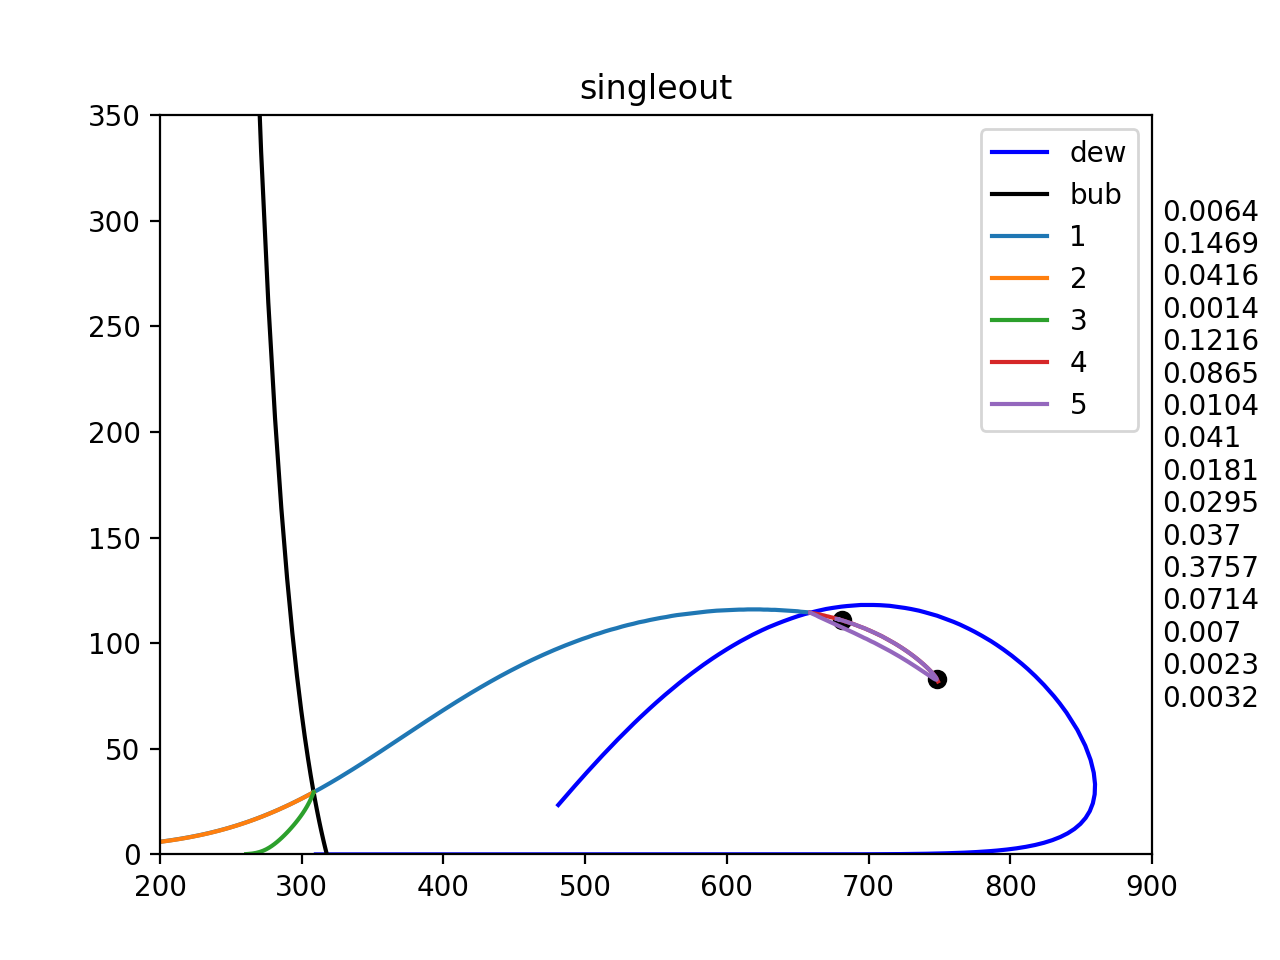
\includegraphics[width=0.7\textwidth]{figs/envelopeex1.png}
    \caption{Envolvente caso $2^*$}
    \label{fig:}
\end{figure}
    
\end{frame}

\begin{frame}[c]
    \frametitle{Gráficos finales}

\begin{figure}[htpb]
    \centering
    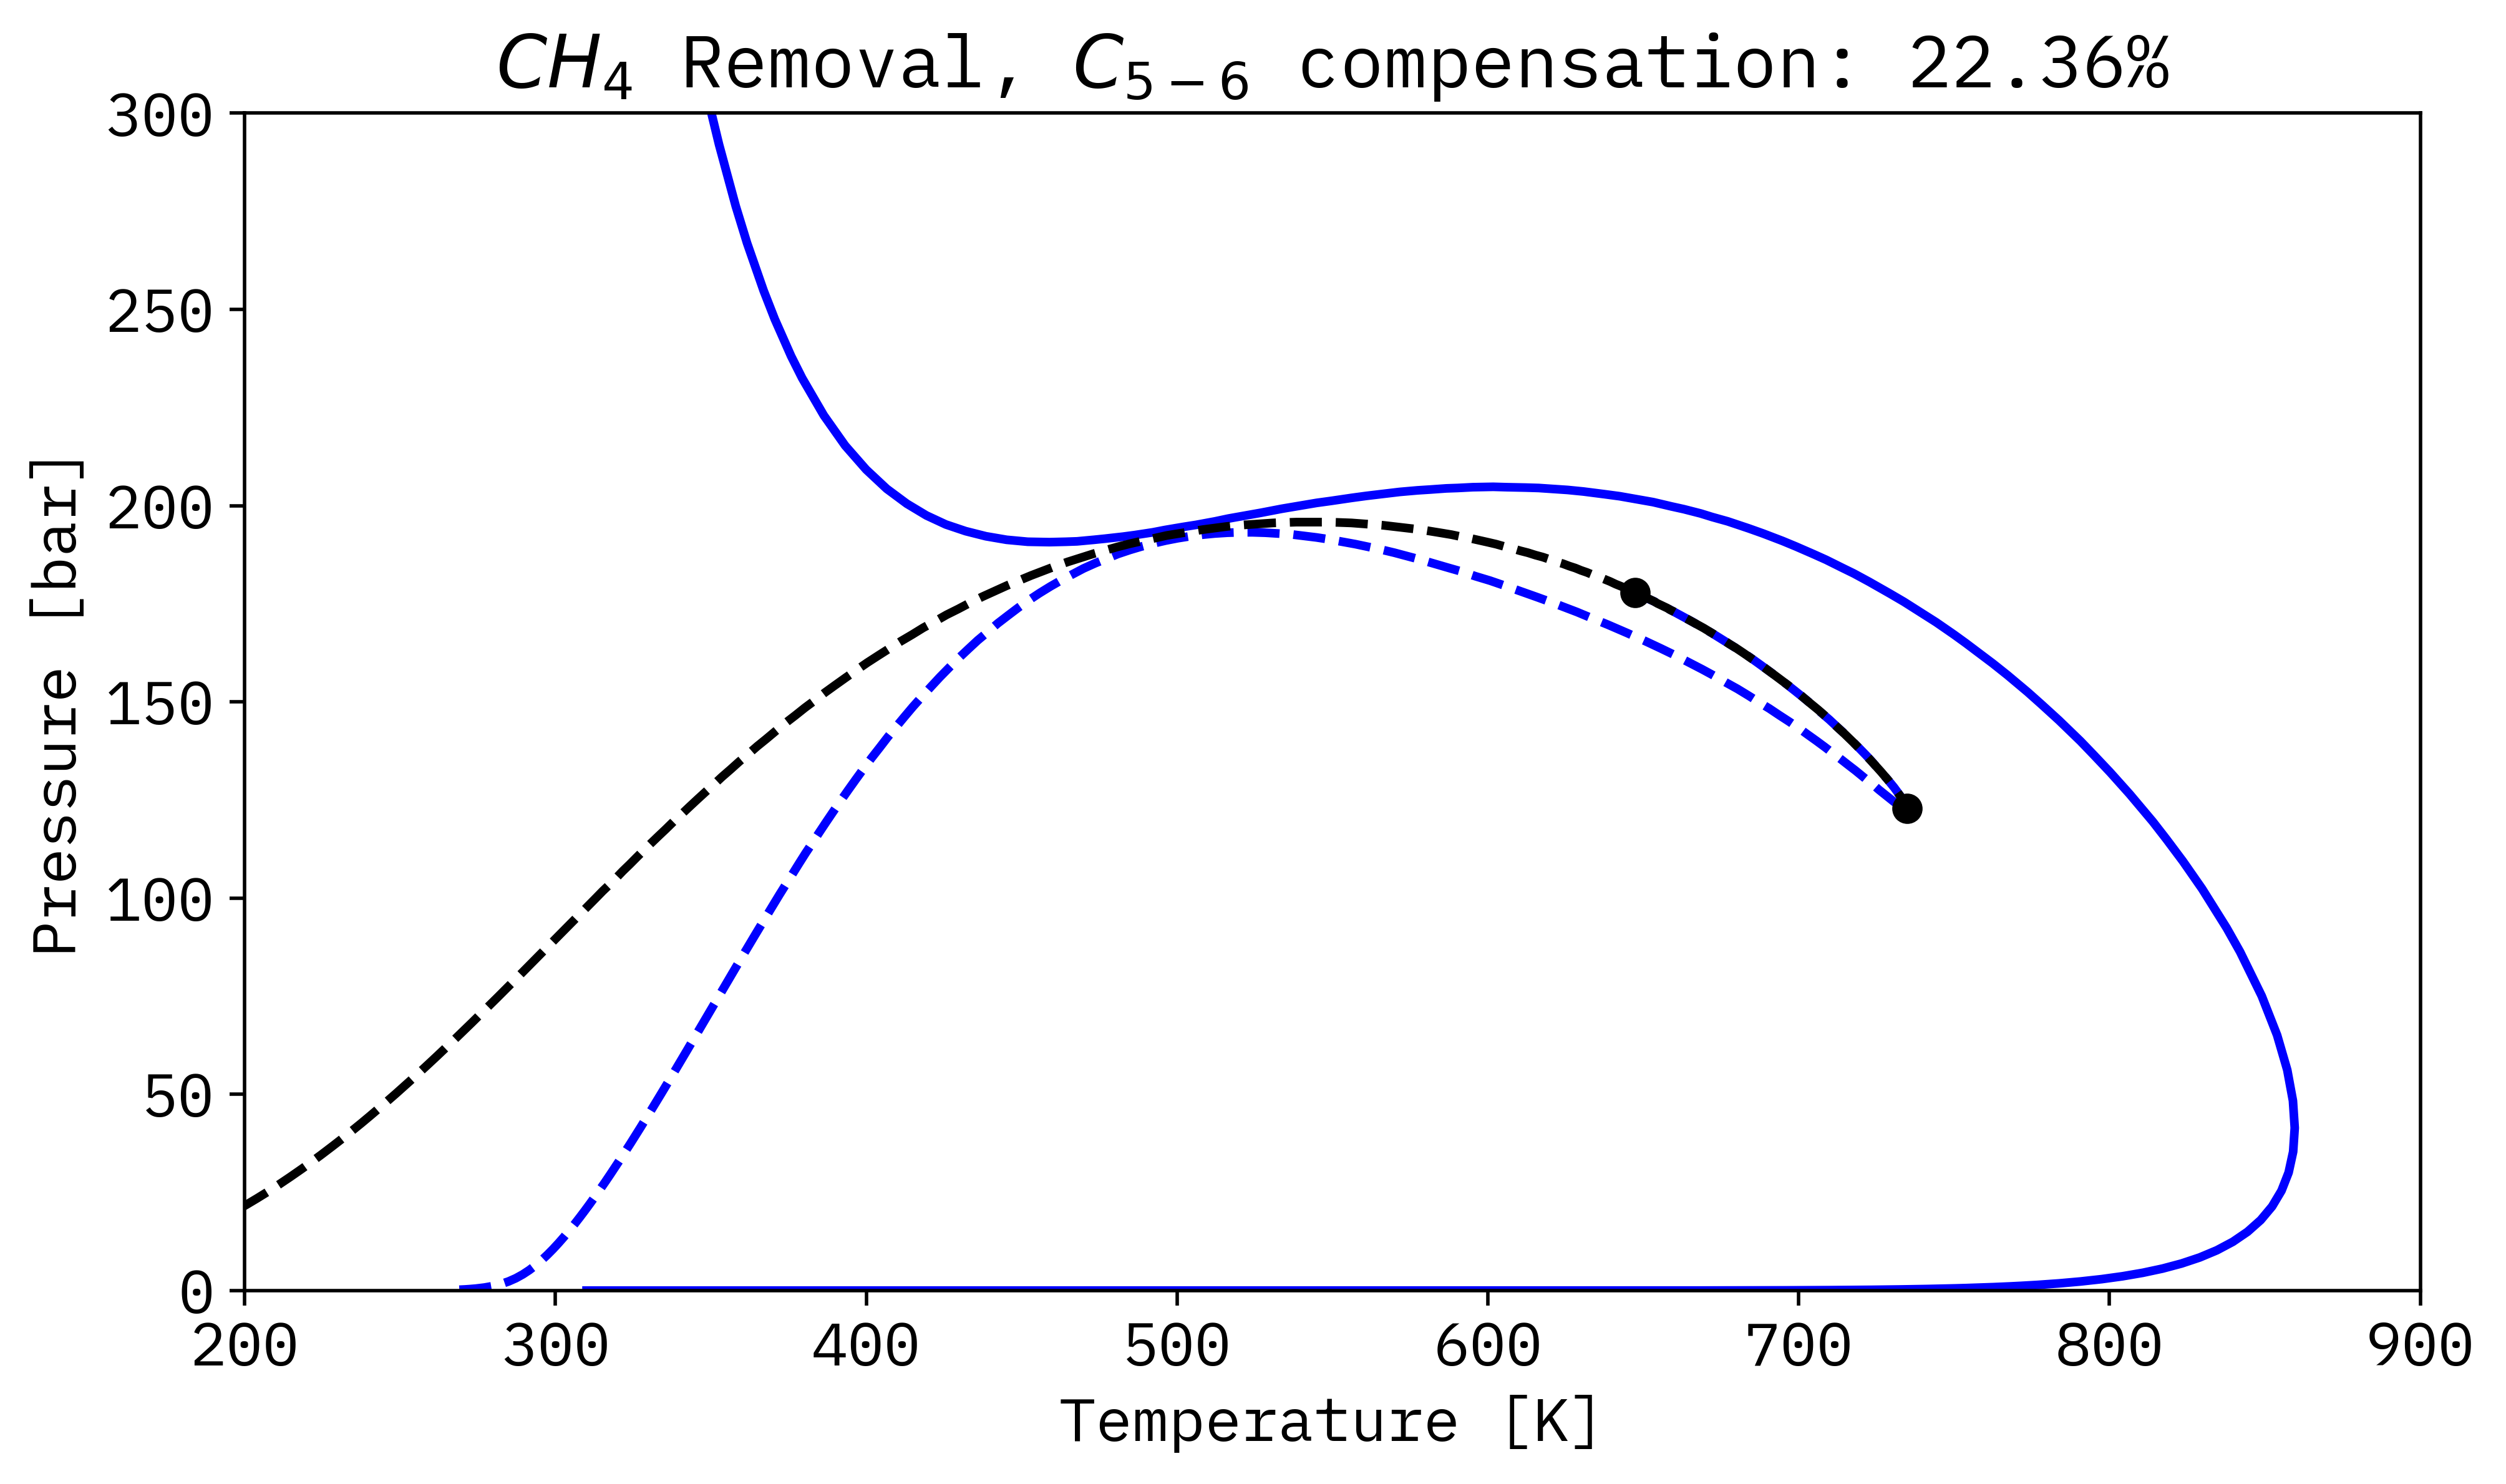
\includegraphics[width=0.8\textwidth]{figs/envelopeex2.png}
    \caption{Envolvente caso 4}
    \label{fig:figs-envelopeex2-png}
\end{figure}
\end{frame}

\titleframe{Muchas gracias!}

\begin{frame}[c]
    \frametitle{Coming soon}

    \begin{itemize}
        \item Fortran Refactoring: Estandarizando códigos...
    \end{itemize}

\end{frame}

\end{document}
